\section{Lois discrètes}

  \subsection{Loi uniforme discrète}
    Soit $X$ une variable aléatoire distribuées selon une loi uniforme discrète sur $\{1,\ldots,n\}$ (voir \cite{uniformlaw}). La distribution est définie comme suit : 
    \begin{equation}
      \forall k\in \{1,\ldots,n\}, \, p(X=k)=\frac 1n \Leftrightarrow X \rightarrow \mathcal U(\{1,\ldots,n\})
      \label{eq:loi_uniforme_discrete}
    \end{equation}


\subsubsection{Exemple - Simulation de la loi uniforme discrète}

  \textbf{Voir code annexe \ref{lst:uniform_distribution}} : \hyperlink{\ref{lst:uniform_distribution}}{Code exemple : Simulation de la loi uniforme discrète}

  \begin{figure}[H]
    \centering
    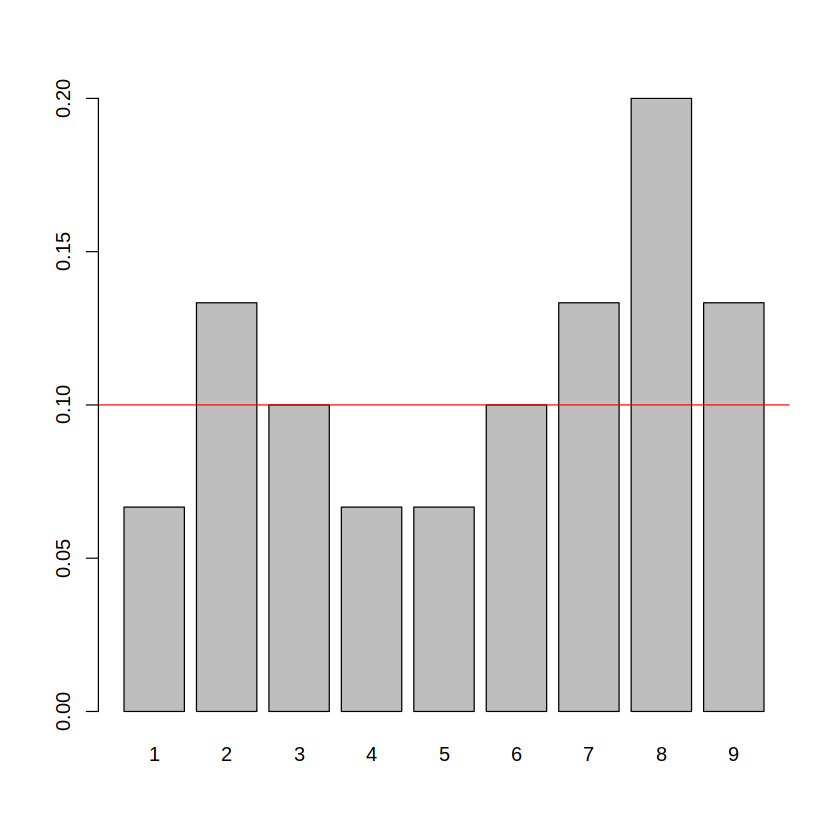
\includegraphics[width=0.28\textwidth]{4_attachments/figures/output3.png}
    \caption{Histogramme de simualtion par loi uniforme discrète avec sa droite de probabilité théorique}
    \label{fig:histogramme_ech}
  \end{figure}

\subsubsection{Analyse des résultats}
  Dans cet exemple (voir code \ref{lst:uniform_distribution}), nous avons simulé un échantillon de taille $30$ selon une loi uniforme discrète $\mathcal{U}(\{1,\ldots,10\})$ (\ref{eq:loi_uniforme_discrete}). Théoriquement, chaque évenement est équiprobable, donc :
  \[
    \forall k\in \{1,\ldots,10\}, \, p(X=k)=\frac 1{10}
  \]

  En analysant les résultats de l'histogramme (Figure~\ref{fig:histogramme_ech}), nous constatons grâce à la droite horizontale rouge représentant la probabilité théorique $p(X)=\frac{1}{10}$, que les fréquences observées varient et ne sont pas toutes égales. Par exemple, 
  \[
    \begin{array}{cc}
      p(X=2) = 0.03 & p(X=4) = 0.23
    \end{array}
  \]
  Cette variation est encore une fois due à la taille réduite de l'échantillon. Les fréquences observées devraient se rapprocher des probabilités théoriques avec un échantillon plus important, conformément à la loi des grands nombres \cite{lawoflargeNumbers}. 
  En conclusion, un échantillon plus important est nécessaire pour démontrer la validité de la loi uniforme discrète de manière plus précise.

\subsection{Loi de Bernoulli}
  Cette loi est notée $\mathcal B(p)$. On dit que $X\leadsto \mathcal B(p)$ si et seulement si $X$ est une variable binaire telle que (voir \cite{bernoulliLaw}) :
  \begin{equation}
    \begin{array}{ccc}
      p(X=1) = p & \text{et} & p(X=0) = 1-p
    \end{array}
  \end{equation}  

  C’est un cas particulier de la loi binomiale avec $n=1$. On peut vérifier facilement par le calcul que $\mathbb E[X]=p$ et $\mathbb V[X]=p(1-p)$.

\subsubsection{Exemple - Simulation de la loi de Bernoulli}

  \textbf{Voir code annexe \ref{lst:bernoulli_distribution}} : \hyperlink{\ref{lst:bernoulli_distribution}}{Code exemple : Simulation de la loi de Bernoulli}

\begin{table}[H]
  \centering
  \begin{tabular}{c c}
    \toprule
    0 & 1 \\
    \midrule
    0.73333 & 0.26667 \\
    \bottomrule
  \end{tabular}
  \caption{Fréquences observées de l'échantillon simulé par la loi de Bernoulli $\mathcal B(0.3)$}
  \label{tab:bernoulli}
\end{table}


\subsubsection{Analyse des résultats}
  Dans cet exemple, nous avons simulé un échantillon de taille $30$ selon une loi de Bernoulli $\mathcal B(0.3)$.
  La loi de Bernoulli est une loi binaire qui ne prend que deux valeurs possibles : $0$ ou $1$.
  Dans notre cas, les fréquences théoriques sont donc:
  \[
    \begin{array}{cc}
      p(\text{Échec}=0) = 0.7 &
      p(\text{Succès}=1) = 0.3
  \end{array}
  \]

  En observant les fréquences (Table~\ref{tab:bernoulli}), la fréquence de succès est de $0.27$ et celle d'échec est de $0.73$.
  Ces fréquences sont proches des probabilités théoriques, avec une légère variation due à la taille de l'échantillon.
  Un échantillon plus grand réduirait cette variation, conformément à la loi des grands nombres \cite{lawoflargeNumbers}.

\subsection{Loi binomiale}
  On dit que $X \leadsto \mathcal B(n,p)$ si $X$ est la somme de $n$ variables de Bernoulli indépendantes de paramètre $p$. $X$ représente le nombre de succès parmi $n$ essais indépendants (voir \cite{binomiallaw}).
  
  Pour résumer, soit $Y \leadsto \mathcal B(p)$ pour $i=1,\ldots,n$ où les $Y_i$ sont indépendantes. On note :
  \begin{equation}
    X = \sum_{i=1}^n Y_i \leadsto \mathcal B(n,p)
  \end{equation}

  Les valeurs possibles pour la variable $X$ sont $\{0,\ldots,n\}$ et 
  \begin{equation}
    \forall k\in\{0,\ldots,n\},\, p_k=p(X=k)=C_n^k p^k (1-p)^{n-k}
  \end{equation}

  \subsubsection{Exemple - Simulation de la loi de binomiale}

    \textbf{Voir code annexe \ref{lst:binomiale_distribution}} : \hyperlink{\ref{lst:binomiale_distribution}}{Code exemple : Simulation de la loi binomiale}
    \begin{table}[H]
      \centering
      \begin{minipage}{0.45\textwidth}
      \centering
      \begin{tabular}{c c c c c c c}
        \toprule
        5 & 6 & 7 & 8 & 9 & 10 \\
        \midrule
        0.02 & 0.06 & 0.30 & 0.36 & 0.16 & 0.09 \\
        \bottomrule
      \end{tabular}
      \caption{Tableau partiel $[5,10]$ des fréquences observées de la simulation binomiale de $p(\text{Succès})=0.8$ et $N=100$ observations}
      \label{tab:binomiale_1}
      \end{minipage}
      \hfill
      \begin{minipage}{0.45\textwidth}
      \centering
      \begin{tabular}{c c c c c c }
        \toprule
        0 & 1 & 2 & 3 & 4 & 6 \\
        \midrule
        0.06 & 0.29 & 0.37 & 0.22 & 0.05 & 0.01 \\
        \bottomrule
      \end{tabular}
      \caption{Tableau partiel $[0,6]$ des fréquences observées de la simulation binomiale de $p(\text{Succès})=0.2$ et $N=100$ observations}
      \label{tab:binomiale_2}
      \end{minipage}
    \end{table}

    \begin{table}[H]
      \centering
      \begin{minipage}{0.45\textwidth}
        \centering
          \begin{tabular}{c c c c c c c}
            \toprule
            5 & 6 & 7 & 8 & 9 & 10 \\
            \midrule
            0.026 & 0.088 & 0.201 & 0.301 & 0.268 & 0.107 \\
            \bottomrule
          \end{tabular}
          \caption{Tableau partiel $[5,10]$ des fréquences théoriques de la loi binomiale $\mathcal{B}(10, 0.8)$, arrondies à 3 décimales}
          \label{tab:binomiale_3}
      \end{minipage}
      \hfill
      \begin{minipage}{0.45\textwidth}
        \centering
        \begin{tabular}{c c c c c c }
          \toprule
          0 & 1 & 2 & 3 & 4 & 6 \\
          \midrule
          0.107 & 0.268 & 0.302 & 0.201 & 0.088 & 0.026 \\
          \bottomrule
        \end{tabular}
        \caption{Tableau partiel $[0,6]$ des fréquences théoriques de la loi binomiale $\mathcal{B}(10, 0.2)$, arrondies à 3 décimales}
        \label{tab:binomiale_4}
      \end{minipage}
    \end{table}

    \subsubsection{Analyse des résultats}
    Dans cet exemple (voir code \ref{lst:binomiale_distribution}), nous avons simulé un échantillon de taille $100$ selon deux lois binomiales : $\mathcal B(10,0.8)$ et $\mathcal B(10,0.2)$. Pour chaque loi, nous avons observé le nombre de succès sur 10 essais répétés 100 fois de manière indépendante.
    
    On peut s'apercevoir que pour la loi $\mathcal B(10,0.8)$, le fréquence la plus élevé est $p(X=8)=0.36$ et pour la loi $\mathcal B(10,0.2)$, la fréquence la plus élevée est $p(X=2)=0.37$. 
    Ce résulat s'explique par la prorpiété d'espérence (moyenne pondérée des valeurs possibles) de la loi binomiale : $\mathbb E[X]=np$.
    \begin{itemize}
      \item Pour la loi $\mathcal B(10,0.8)$, on s'attend à avoir $\mathbb E[X]=np=10*0.8=8$ succès en moyenne.
      \item Pour la loi $\mathcal B(10,0.2)$, on s'attend à avoir $\mathbb E[X]=np=10*0.2=2$ succès en moyenne.
    \end{itemize}

    En comparant les fréquences observées (Tableaux~\ref{tab:binomiale_1} et \ref{tab:binomiale_2}) avec les fréquences théoriques (Tableaux~\ref{tab:binomiale_3} et \ref{tab:binomiale_4}), nous remarquons une bonne concordance, bien que des variations existent en raison de la taille du nombre de répétitons.

    Pour vérifier cela, si nous augmentons la taille de l'échantillon à $N=10000$, les fréquences observées se rapprochent encore plus des fréquences théoriques :
    \begin{itemize}
      \item Pour la loi $\mathcal B(10,0.8)$ : $p(X=8)=0.3026$
      \item Pour la loi $\mathcal B(10,0.2)$ : $p(X=2)=0.3033$
    \end{itemize}


    \subsection{Loi Géométrique}  
      On dit que $X$ suit une loi géométrique $\mathcal G(p)$ avec $ 0 < p < 1$
      On répète, de façon indépendante, une même expérience (qui a une probabilité $p$ de réussite et une probabilité $q=1-p$ d’échec) et on note $X$ le rang du premier succès (voir \cite{geometriclaw}).
      Les valeurs prises par $X$ sont donc $X(\Omega) = N*$ et les probabilités associés sont:
      \begin{equation}
        \forall k\in\mathbb N^\star,\, p_k=P(X=k) = (1-p)^{k-1}p = q^{k-1}p
        \label{eq:loi_geometrique}
      \end{equation}

      \subsubsection{Exemple - Simulation de la loi géométrique}

      \textbf{Voir code annexe \ref{lst:geometric_distribution}} : \hyperlink{\ref{lst:geometric_distribution}}{Code exemple : Simulation de la loi géométrique}

      \begin{figure}[H]
        \centering
        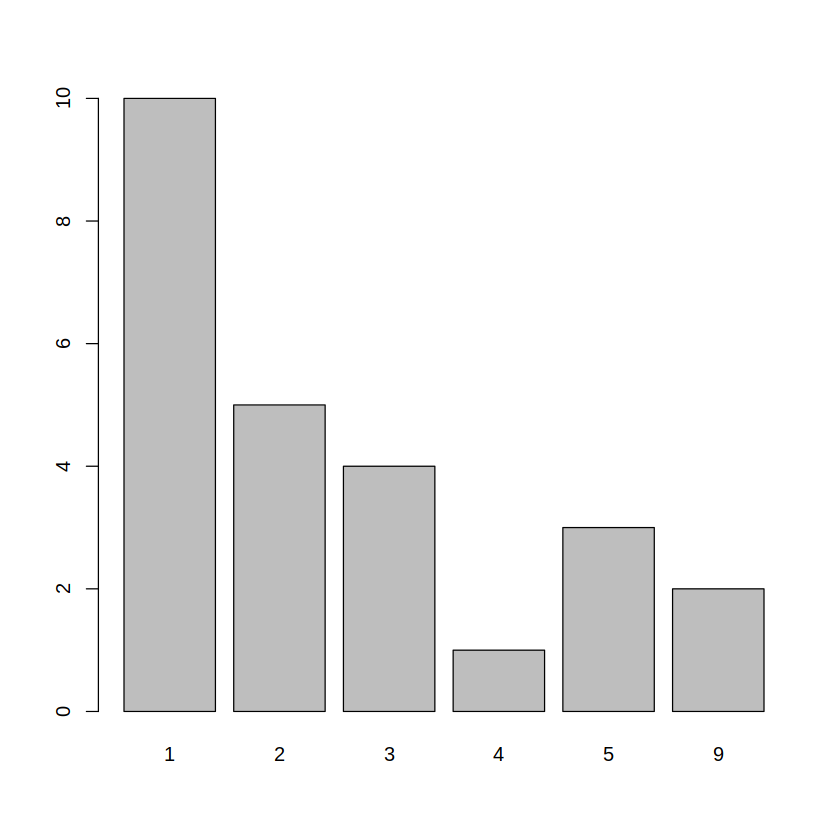
\includegraphics[width=0.28\textwidth]{4_attachments/figures/output4.png}
        \caption{Histogramme de simualtion par loi géométrique avec une probabilité $p(X= \text{Succès})=0.3$ et une taille d'échantillon de $25$}
        \label{fig:histogramme_ech}
      \end{figure}

    \subsubsection{Analyse des résultats}
    Dans cet exemple (voir code \ref{lst:geometric_distribution}), nous avons simulé un échantillon de taille $25$ selon une loi géométrique $\mathcal G(0.3)$.
    Comme nous pouvons le remarquer dans l'histogramme (Figure~\ref{fig:histogramme_ech}), les fréquences observés sont décroissantes, ce qui est conforme à la loi géométrique (\ref{eq:loi_geometrique}). Par exemple :
    \[
      \begin{array}{ll}
        p(X=1) &= \frac{10}{25} = 0.4 \approx (1-0.3)^{1-1}0.3 = 0.3 \\ 
        p(X=2) &= \frac{5}{25} = 0.2 \approx (1-0.3)^{2-1}0.3 = 0.21
      \end{array}
    \]

    \subsection{Loi de Poisson}
      On dit que $X$ suit une loi de Poisson $\mathcal P(\lambda)$ avec $\lambda > 0$.
      On peut voir cette loi comme la loi des événements rares. 
      Cette loi est une approximation de la loi binomiale, $\mathcal B(n,p)$ lorsque n est grand et p petit. 
      On pose alors $\lambda=np$. En pratique, on dit que cette approximation est bonne dès que $n>20$ et $p<=0.1$ et $np<=5$ (voir \cite{poissonlaw}).

      Les valeurs possibles pour $X$ sont dans $N$ et les probabilités associées : 
      \begin{equation}
        \forall k\in \mathbb N,\, p_k=P(X=k)=e^{-\lambda}\dfrac{\lambda^k}{k!}
        \label{eq:loi_poisson}
      \end{equation}

    \subsubsection{Exemple - Simulation de la loi Poisson}

      \textbf{Voir code annexe \ref{lst:poisson_distribution}} : \hyperlink{\ref{lst:poisson_distribution}}{Code exemple : Simulation de la loi Poisson}

      \begin{figure}[H]
        \centering
        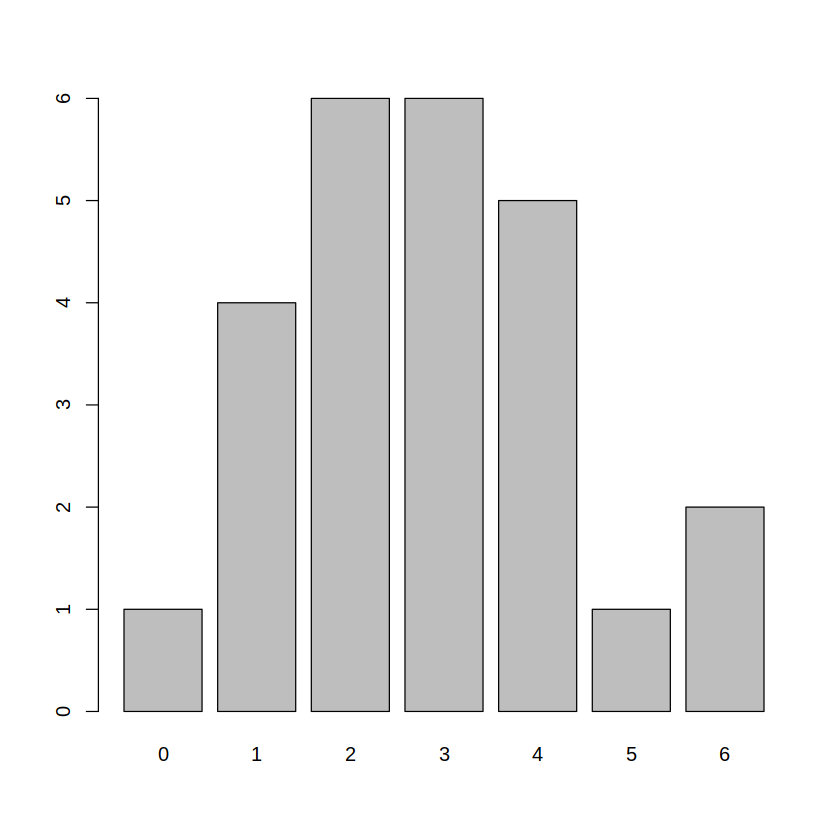
\includegraphics[width=0.28\textwidth]{4_attachments/figures/output5.png}
        \caption{Histogramme de simualtion par loi poisson avec un paramètre $\lambda=3$ et une taille d'échantillon de $25$}
        \label{fig:histogramme_poisson}
      \end{figure}

      \subsubsection{Analyse des résultats}
      Dans cet exemple, nous avons simulé un échantillon de taille $n=25$ selon une loi de Poisson $\mathcal P(3)$. Ce qui signifie $\lambda=3=np$ donc cet exemple à une probabilité de succès de $p=0.12$.
      On se trouve bien dans le cas où $n>20$ et $p<=0.1$ et $np<=5$.

      En observant l'histogramme (Figure~\ref{fig:histogramme_poisson}), nous constatons que les fréquences observées sont conformes à la loi de Poisson (\ref{eq:loi_poisson}). Par exemple :
      \[
        \begin{array}{ll}   
          p(X=0) &= \frac{1}{25} = 0.04 \approx e^{-3}\dfrac{3^0}{0!} = 0.049 \\
          p(X=1) &= \frac{4}{25} = 0.16 \approx e^{-3}\dfrac{3^1}{1!} = 0.149 \\ 
          p(X=2) &= \frac{6}{25} = 0.24 \approx e^{-3}\dfrac{3^2}{2!} = 0.224
        \end{array}
      \]

      Nous pouvons observer grâce à la Figure \ref{fig:poisson_binomiale} ci-dessous que la loi Poisson converge est une approximation de la loi binomiale pour $n$ grand et $p$ petit.
      \begin{figure}[H]
        \centering
        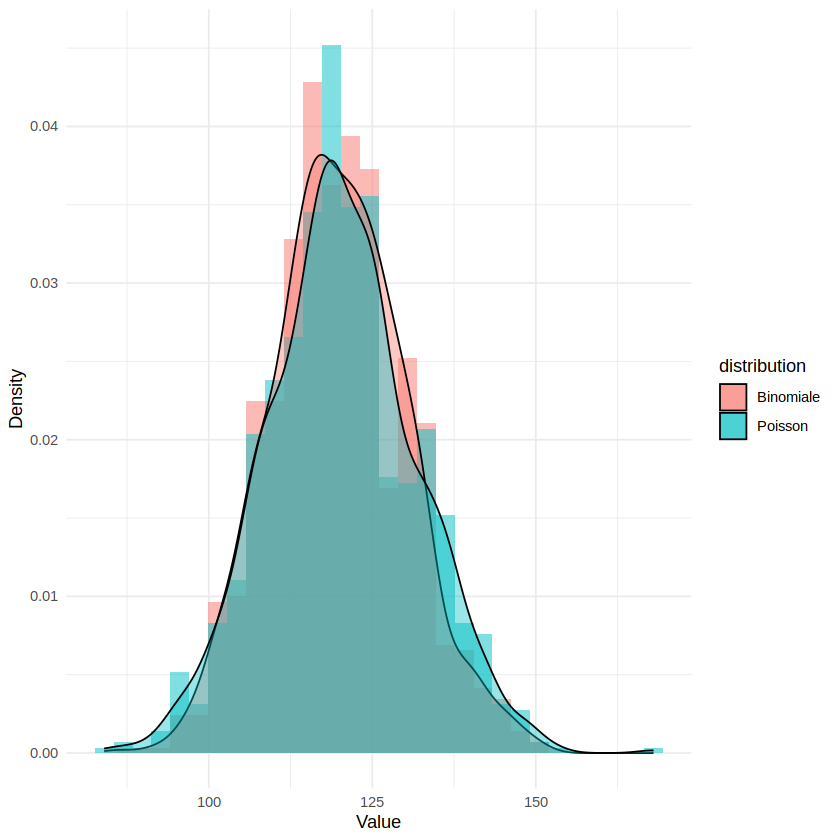
\includegraphics[width=0.35\textwidth]{4_attachments/figures/output6.png}
        \caption{Comparaison de la loi de Poisson et de la loi binomiale pour $n=1000$ et $p=0.12$}
        \label{fig:poisson_binomiale}
      \end{figure}

      Lorsque l'on fait varier le paramètre $\lambda$ de la loi de Poisson, on peut observer que la distribution se déplace vers la droite (Figure~\ref{fig:poisson_lambda}). Cela s'explique par le fait que $\lambda$ est l'espérance de la loi de Poisson, dans le tableau ci-dessous Table \ref{tab:poisson_lambda}, on peut voir que pour $\lambda=2$ la médiane et la moyenne sont égales à $2$ (ou très proche en fonction de la taille de l'échantillon $n$)
      Alors que pour $\lambda=5$, la moyenne est de $5$ et la médiane est de $5$.

      \begin{table}[H]
        \centering
        \begin{minipage}{0.45\textwidth}

          \begin{figure}[H]
            \centering
            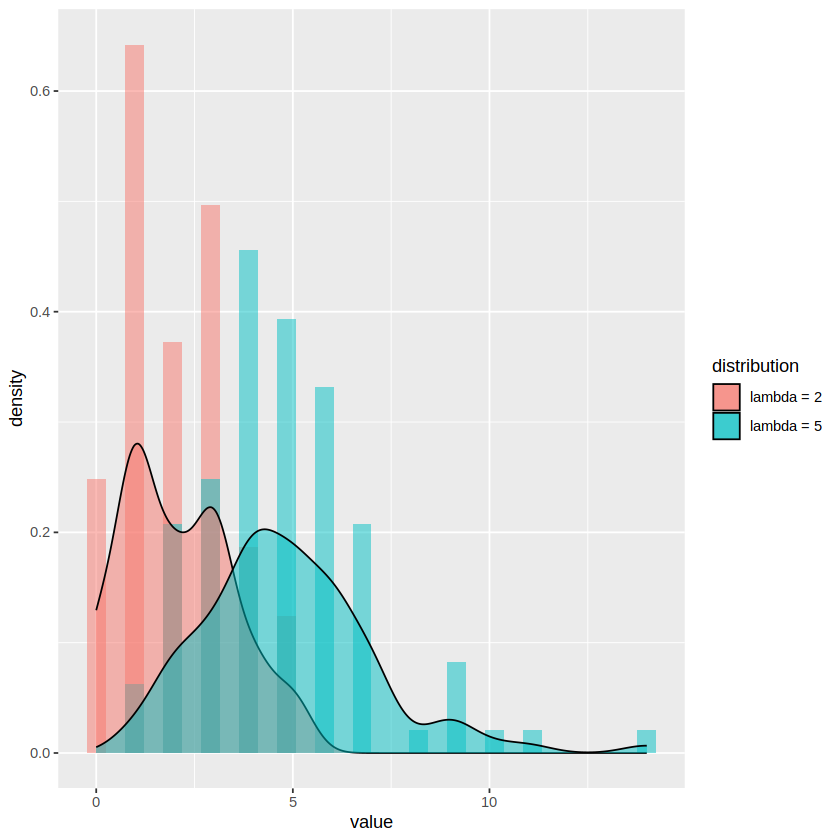
\includegraphics[width=0.9\textwidth]{4_attachments/figures/output7.png}
            \caption{Comparaison de la loi de Poisson selon le paramètre $\lambda$}
            \label{fig:poisson_lambda}
          \end{figure}
        \end{minipage}
        \hfill
        \begin{minipage}{0.45\textwidth}
          \centering
          \begin{table}[H]
            \centering
            \begin{tabular}{c c c c c c c}
              \toprule
              $\lambda$ & $n$ & Moyenne & Médiane \\
              \midrule
              2 & 100 & 2.05 & 2.00 \\
              5 & 100 & 4.87 & 5.00 \\
              \bottomrule
            \end{tabular}
            \caption{Comparaison des paramètres de la loi de Poisson pour $\lambda=2$ et $\lambda=5$}
            \label{tab:poisson_lambda}
          \end{table}
        \end{minipage}
      \end{table}